% =====================================================================
% 3. Training loop and evaluation code (MLLB, Maria Martinez)
% T7 (own: src/metrics.py, src/runlog.py, src/compare.py, make_numbers.py),
% T8 (shared: src/train.py, src/tasks.py). DECISIONS D4, D14.
% =====================================================================
\section{Training and evaluation}\label{sec:mllb-training}

The training loop was written by Oriana and me together (task T8); the evaluation module, the run logs,
the comparison tool and the script that turns the logs into the numbers of the reports are mine (T7).

\subsection{The training loop}

Listing~\ref{lst:train} is the core of the loop. Each iteration performs the five steps of PyTorch
training: clear the old gradients, forward pass, loss, backpropagation, update.
\begin{itemize}[leftmargin=1.2em,itemsep=1pt]
  \item \texttt{model.train()} and \texttt{model.eval()} switch dropout (and batch norm) between training
        and evaluation behaviour; evaluation also runs under \texttt{torch.no\_grad()}, so no graph is built
        and memory is saved.
  \item \textbf{Gradient clipping goes between \texttt{backward()} and \texttt{step()}}: the gradients must
        exist before their norm can be limited, and they must be limited before the optimiser uses them.
        All my recurrent and Transformer configurations clip the total norm at \rnnGradClip{}.
  \item \texttt{loss.item()} turns the loss into a Python number; accumulating the tensor itself would keep
        each batch's graph alive.
  \item In evaluation, the losses are summed and divided by the number of terms at the end, so the epoch
        loss is the exact mean over the split even when the last batch is smaller.
\end{itemize}

\lstinputlisting[firstnumber=101,caption={One training epoch and the evaluation pass (\texttt{src/train.py}).},label={lst:train}]{common/code/train_one_epoch.py}

The loop does not know the problem. Everything specific comes from a \emph{task} object: the loss, the
metrics accumulated batch by batch, and the metric that decides early stopping with its direction. For the
classifiers the loss is \texttt{binary\_cross\_entropy\_with\_logits} on the five logits
(Listing~\ref{lst:loss}), which combines the sigmoid and the cross-entropy in one numerically stable
operation; that is why no model ends in a sigmoid. The same loop, with a next-token task, trains Oriana's
generators.

\lstinputlisting[firstnumber=91,caption={Multi-label loss of the classification task (\texttt{src/tasks.py}).},label={lst:loss}]{common/code/multilabel_loss.py}

\paragraph{Early stopping.} After every epoch the model is evaluated on validation. When the validation
macro AUROC improves, a copy of the weights is kept on the CPU: a plain reference to
\texttt{model.state\_dict()} would change as training continues. After 5 epochs without improvement,
training stops and the best weights are loaded back. The optimiser receives only the parameters with
\texttt{requires\_grad=True}, so the frozen layers of the transfer experiments need no special code.

\paragraph{Reproducibility on the GPU.} Python, NumPy and PyTorch are seeded before the model is built, and
cuDNN runs in deterministic mode. For the recurrent and attention models, the PyTorch documentation of
\texttt{nn.LSTM} warns that RNN functions can be non-deterministic on some CUDA versions and suggests
setting \texttt{CUBLAS\_WORKSPACE\_CONFIG=:4096:2}; my experiment scripts set it before CUDA starts and
write it to every log. With it, the final runs of both of my blocks reproduced their validation runs
exactly (same validation AUROC and best epoch), so the GPU runs were deterministic in practice.

\paragraph{Training curves.} Figures~\ref{fig:rnn_curves} and~\ref{fig:transformer_curves} are the
diagnostic curves of my blocks: training and validation loss of the baselines, validation AUROC per epoch,
and the comparisons that concern optimisation (1000 raw steps against 100 frames; Pre-LN against Post-LN).
The LSTM over 1000 raw steps starts much more slowly than over frames, and both baselines reach their best
validation AUROC early and then overfit, which is what early stopping is for.

% Shared float (common/make_floats.py). Figure: figures/rnn_curves.pdf
\begin{figure}[htbp]
\centering
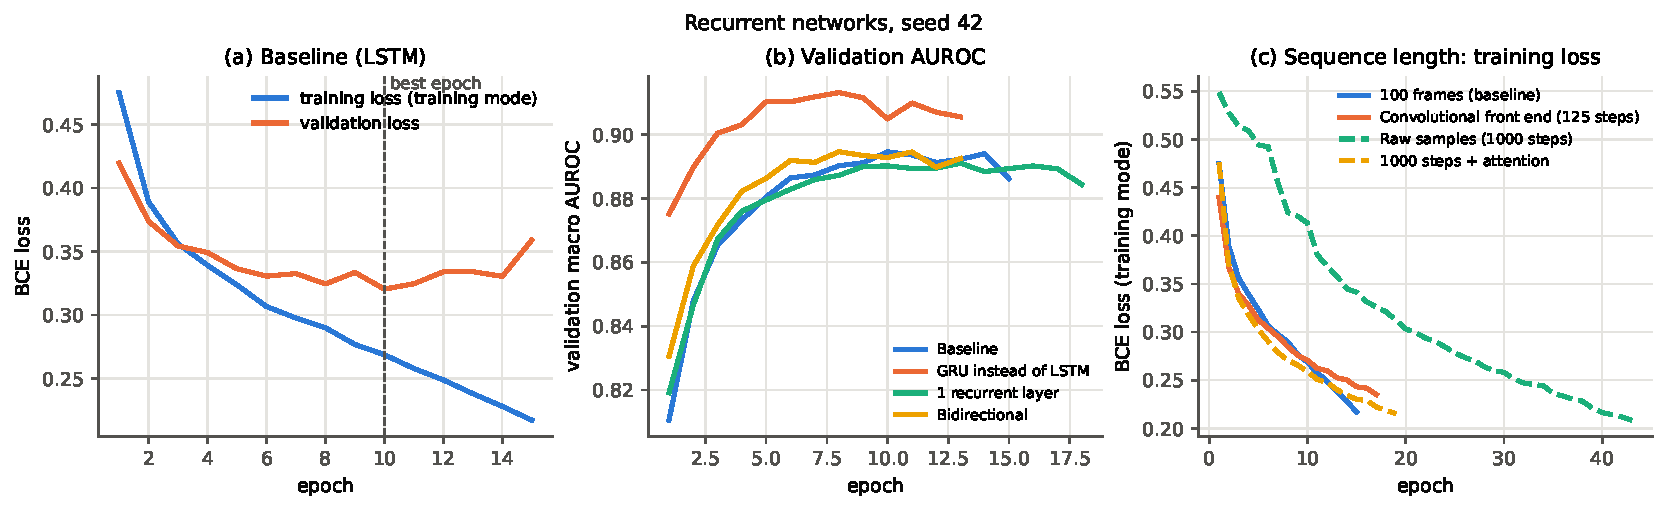
\includegraphics[width=\textwidth,height=0.42\textheight,keepaspectratio]{figures/rnn_curves.pdf}
\caption[Recurrent networks: learning curves]{Recurrent networks, seed 42. (a) LSTM baseline losses. (b) Validation macro AUROC of the baseline, GRU, one recurrent layer and bidirectional LSTM. (c) Training loss with 100 frames, the convolutional front end, 1000 raw steps and 1000 steps with attention.}
\label{fig:rnn_curves}
\end{figure}

% Shared float (common/make_floats.py). Figure: figures/transformer_curves.pdf
\begin{figure}[htbp]
\centering
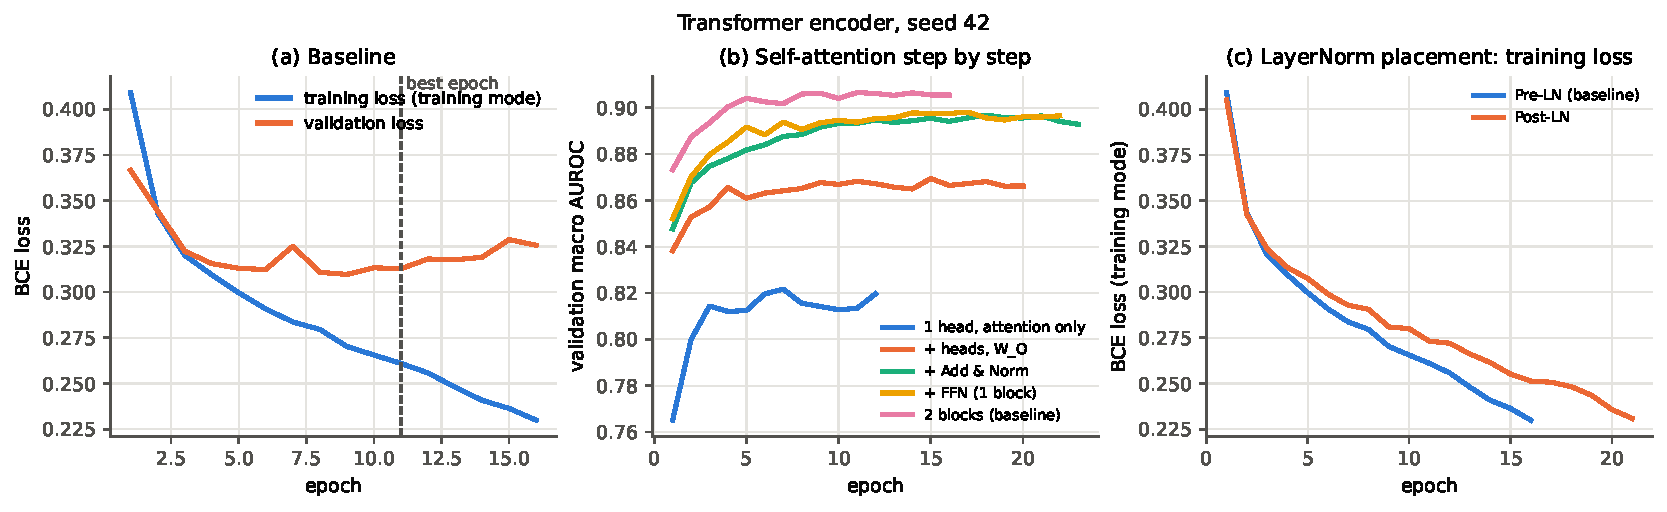
\includegraphics[width=\textwidth,height=0.42\textheight,keepaspectratio]{figures/transformer_curves.pdf}
\caption[Transformer: learning curves and self-attention step by step]{Transformer encoder, seed 42. (a) Baseline losses. (b) Self-attention step by step: validation macro AUROC from one single-head attention layer to two full blocks. (c) Training loss with Pre-LN and Post-LN.}
\label{fig:transformer_curves}
\end{figure}


\subsection{Evaluation code}

\paragraph{Metrics.} Probabilities are \texttt{sigmoid(logits)}, computed outside the model. The AUROC of
each class comes from scikit-learn and the macro AUROC is their plain mean. For F1, each class gets the
threshold of the grid 0.01--0.99 that maximises its F1 on validation (lowest threshold on ties), and the
same thresholds are applied to test.

\paragraph{Patient bootstrap.} Listing~\ref{lst:boot} draws the resamples. Patients, not records, are drawn
with replacement; \texttt{np.bincount} counts how many times each patient was drawn and \texttt{np.repeat}
repeats all of that patient's records as many times. Because the draws depend only on the patient
identifiers and the seed, every model evaluated on the same split sees exactly the same resamples. A
resample in which a class has no positive or no negative record (AUROC undefined) is discarded and counted
in the log.

\lstinputlisting[firstnumber=101,caption={Patient-level bootstrap resamples (\texttt{src/metrics.py}).},label={lst:boot}]{common/code/patient_bootstrap.py}

\paragraph{Paired difference.} Listing~\ref{lst:paired} uses those same resamples to compute the interval of
the difference in macro AUROC between two models on the same records. It needs both models' predictions in
the same record order, which is why every run saves its probabilities with the record and patient
identifiers, and why \texttt{python -m src.compare RUN\_A RUN\_B} refuses two runs whose records differ.

\lstinputlisting[firstnumber=164,caption={Paired bootstrap difference of two models (\texttt{src/metrics.py}).},label={lst:paired}]{common/code/paired_bootstrap.py}

\subsection{Run logs and numbers of the reports}

Every run is named \texttt{<model>\_<tag>\_s<seed>\_<date-time>} and writes three files: a JSON log
(configuration, seed, data description, curves, best epoch, results per split with intervals, parameter
counts, software versions, git commit and whether the code under \texttt{src/} had uncommitted changes), the
predictions (\texttt{.npz}) and the best weights (not committed). The test fold is evaluated only with
\texttt{--final}, and a second final run with the same model, tag and seed is refused.

\texttt{report/runs.json} maps a short alias to each log or block summary allowed in a report, and
\texttt{report/make\_numbers.py} turns every scalar of those logs into a LaTeX macro. Macro names can only
contain letters, so the key is cut at underscores and at letter--digit boundaries and digits are spelled
out: the mean test macro AUROC of the final RNN is \verb|\rnnFinalTestMacroAurocMean| and prints
\rnnFinalTestMacroAurocMean{}. A report therefore cannot contain a number that is not in a log, and a
re-run updates every table and sentence at once.
